\documentclass[12pt, letterpaper]{article}
\usepackage[utf8]{inputenc}
\usepackage[margin=1in]{geometry}
\usepackage{graphicx}
\usepackage{fancyhdr}
\usepackage{biblatex}
\usepackage{hyperref}
\usepackage[section]{placeins}
\addbibresource{references.bib}

\setlength{\parskip}{1em}
\setlength{\parindent}{0em}


\title{Parallel KNN}
\author{Charisios Vogiatzis}

\begin{document}

\maketitle
\begin{center}
    \huge{Parallel kNN}
    
    \large{Charisios Vogiatzis}
\end{center}

\href{https://github.com/charisvt/PDS-KNN}{Code on Github}\\

\rule{\textwidth}{0.5pt}

\section{Introduction}
This is an implementation of the all-kNN algorithm in a sequential version (V.0) and a parallel version (V.1) using the MPI library. 
The goal is to provide a scalable optimised algorithm that can process huge amounts of data, thus providing a way to bypass memory limitations imposed by the execution on a single host.

\subsection{V.0 Sequential}
The algorithm we are implementing is calculating the (squared) Euclidean Distance: 

\begin{equation}
    D = (X \odot X)\, e\, e^{T} - 2\, X\, Y^{T} + e\, e^{T}(Y \odot Y)^{T}
\end{equation}

We are using the OpenBLAS library to perform the matrix multiplication $XY^{T}$.\\
We are using kselect to calculate the kNN with time complexity of O(n) (*for big n).
OpenMP API is used to perform same-host parallelisation in the form of threads to accelerate the execution of certain parts of the algorithm.


\subsection{V.1 Parallel}
The parallel version of the algorithm uses a ring (round-robin) topology and splits the total amount of data into P nodes, forming blocks. 
Each node is tasked with a block query X, calculates kNN with corpus Y and then forwards Y to the next node, for a total of P steps. 
Since on the first step the query and corpus data are the same, we only need a total of P-1 exchanges.

\begin{figure}[h]
    \centering
    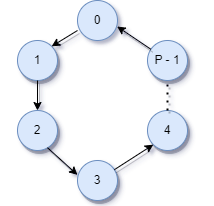
\includegraphics[height=4cm]{ring.png}
    \caption{Ring Topology}
    \label{fig:img-1}
\end{figure}

As a scheduling scheme to facilitate sending data and calculating kNN we are using the following.
\begin{figure}[h]
    \centering
    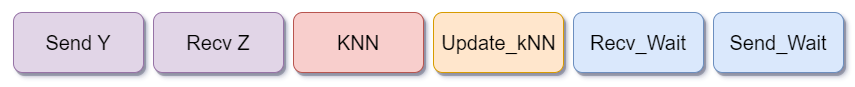
\includegraphics[width=1\linewidth]{Flow diagram 2.png}
    \caption{Scheduling}
    \label{fig:img-2}
\end{figure}
\\
We begin forwarding our data to the next node and then proceed to calculate kNN.
Send Y and Recv Z are non-blocking operations, allowing us to run the kNN algorithm while sending and receiving data and thus hide communication costs. 
Recv Wait and Send Wait are blocking operations and provide synchronisation. On the first step we ommit the Update kNN block and on the last step we omit the communications blocks. 
After all steps are completed, nodes $[1 - (p-1)]$ send their results to node $[0]$ to sequentially write them to the output file in the correct order to keep track of index information.
\begin{figure}[h]
    \centering
    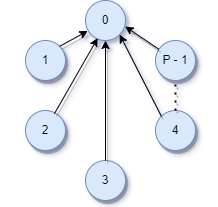
\includegraphics[height=4cm]{ring-many-to-1.png}
    \caption{Data gathering}
    \label{fig:img-3}
\end{figure}

\section{Results}
\textbf{Sequential}\\[0.5ex]
\begin{tabular}{|c|c|c|}
\hline
\textbf{Size} & \textbf{V0} \\ [0.5ex] 
\hline\hline
1000 & 0.014s  \\ 
\hline
8000 & 0.165s \\
\hline
15625 & 0.584s \\
\hline
\end{tabular}
\section{Disclaimer}
The final parallel version currently has a bug which I could not fix in time. It works properly for 1 node but crashes when run on more. A previous stable version did not crash but produced some bad intermediate blocks in the results which I discovered too late, probably due to an unresolved race condition. I decided to not display these time measurements regarding that version since the results were partly incorrect.
The algorithm uses $O(n^2)$ memory since the Distances matrix is size $M x M$. 
One solution to this is to block Y corpus to calculate the matrix in batches so the total size can be reduced to $M x (M/c)$ where $c$ can be chosen accordingly to produce the desired maximum allowed memory block. 
This however has not been implemented here.

\section{Resources}
You can find the different versions on the different branches on the \href{https://github.com/charisvt/PDS-KNN}{Github repo} along with some helper programs and the LaTeX source code for this document.
The resources are under the \href{https://www.mit.edu/~amini/LICENSE.mdMIT}{MIT licence}.

\section{Acknowledgement}
This work uses the GPT-3 model, which is a state-of-the-art \href{https://chat.openai.com/chat}{language model} developed by OpenAI.
\end{document}
